\documentclass[tikz, convert={outfile=\jobname.png}]{standalone}
\usepackage[utf8]{inputenc}
\usetikzlibrary{calc,shapes.multipart,chains,scopes,arrows}

\newcommand{\connectlist}[2]{%
  \draw[*->] let \p1 = (#1.two), \p2 = (#1.center) in (\x1, \y2) -- (#2)}

\newcommand{\oldconnectlist}[2]{%
  \draw[dashed, *->, color=gray] let \p1 = (#1.two), \p2 = (#1.center) in (\x1, \y2) -- (#2)}

\newcommand{\newconnectlist}[2]{%
  \draw[->, color=red]
    let \p1 = (#1.two), \p2 = (#1.center) in
    (\x1, \y2) -- ++(0, -0.5) -| (#2)}

\newcommand{\connectpointer}[2]{%
  \draw[->] (#1) -- (#2)}

\newcommand{\oldconnectpointer}[2]{%
  \draw[dashed, ->, color=gray] (#1) -- (#2)}

\newcommand{\newconnectpointer}[2]{%
  \draw[->, color=red] (#1) -- (#2)}

\begin{document}
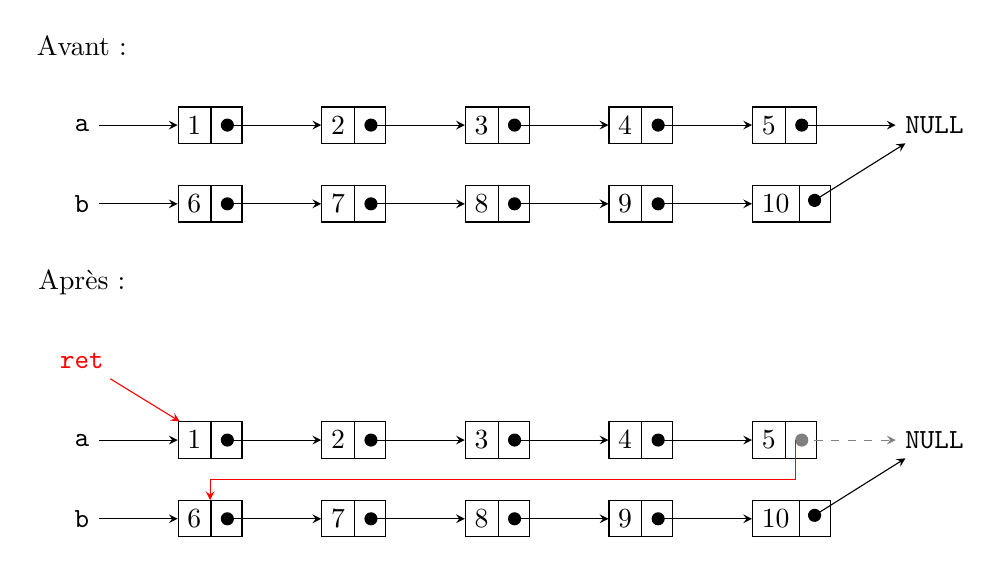
\begin{tikzpicture}[
    list/.style={rectangle split, rectangle split parts=2, draw,
    rectangle split horizontal}, >=stealth]
  \node (before) {Avant~:};
  {[start chain]
    \node[on chain, below of=before] (a) {\texttt{a}};
    \node[list, on chain] (n1) {1};
    \node[list, on chain] (n2) {2};
    \node[list, on chain] (n3) {3};
    \node[list, on chain] (n4) {4};
    \node[list, on chain] (n5) {5};
    \node[on chain] (nil) {\texttt{NULL}};

    \connectpointer{a}{n1};
    \connectlist{n1}{n2};
    \connectlist{n2}{n3};
    \connectlist{n3}{n4};
    \connectlist{n4}{n5};
    \connectlist{n5}{nil};}

  {[start chain]
    \node[on chain, below of=a] (b) {\texttt{b}};
    \node[list, on chain] (na) {6};
    \node[list, on chain] (nb) {7};
    \node[list, on chain] (nc) {8};
    \node[list, on chain] (nd) {9};
    \node[list, on chain] (ne) {10};

    \connectpointer{b}{na};
    \connectlist{na}{nb};
    \connectlist{nb}{nc};
    \connectlist{nc}{nd};
    \connectlist{nd}{ne};
    \connectlist{ne}{nil};}

  \node[below of=b] (after) {Après~:};
  {[start chain]
    \node[below of=after, color=red] (ret) {\texttt{ret}};
    \node[on chain, below of=ret] (a) {\texttt{a}};
    \node[list, on chain] (n1) {1};
    \node[list, on chain] (n2) {2};
    \node[list, on chain] (n3) {3};
    \node[list, on chain] (n4) {4};
    \node[list, on chain] (n5) {5};
    \node[on chain] (nil) {\texttt{NULL}};

    \newconnectpointer{ret}{n1};
    \connectpointer{a}{n1};
    \connectlist{n1}{n2};
    \connectlist{n2}{n3};
    \connectlist{n3}{n4};
    \connectlist{n4}{n5};
    \oldconnectlist{n5}{nil};}

  {[start chain]
    \node[on chain, below of=a] (b) {\texttt{b}};
    \node[list, on chain] (na) {6};
    \node[list, on chain] (nb) {7};
    \node[list, on chain] (nc) {8};
    \node[list, on chain] (nd) {9};
    \node[list, on chain] (ne) {10};

    \connectpointer{b}{na};
    \newconnectlist{n5}{na};
    \connectlist{na}{nb};
    \connectlist{nb}{nc};
    \connectlist{nc}{nd};
    \connectlist{nd}{ne};
    \connectlist{ne}{nil};}
\end{tikzpicture}

\end{document}
